\chapter{Introduction}
\label{cha:intro}

\section{Motivation}
\label{sec:motivation}
Constructing an end-to-end differentiable network to solve constrained optimization problems is one of the most elusive
and long-standing challenges in Artificial Intelligence.  Modern deep learning models have produced many insightful achievements in various domains with different functional layers and nodes. Most state-of-the-art network structures perform well in solving computer vision tasks~\citep{SK:14, HK:16, SM:18} such as image recognition, segmentation and reconstruction. These neural network models are constructed with parametrized processing layers~\citep{SG:19}, which pass the data through explicitly defined nodes. These nodes are usually composed of a differentiable forward function and the output is well-defined. Also, the input of these tasks is usually the image, which can be analyzed in matrix form and the transformation between layers is continuous. However, what if the problems have discrete logical relationships? How do we capture these constraints? Figure~\ref{fig:sudoku-table} demonstrates several 9 $\times$ 9 Sudoku puzzles and their corresponding solutions from the Kaggle competition dataset~\citep{RR:19}, where unknowns are zeros in the puzzles. Obviously, the relationship between each value in the puzzle is discrete, since all rows, columns and blocks are constrained with different rules. To optimize such logic-based puzzle games, many researchers have put decades of efforts to approach constrained optimization problems from various aspects, including:
\begin{itemize}
    \item \textbf{Existence of optimizers. }The solution of the problem is defined based on the existence of optimizers, which requires our model to verify. For example, a normal 9 $\times$ 9 Sudoku puzzle has at least one solution satisfying all rules. That means if we transfer it to a mathematical constrained optimization problem, there is a global optimizer or multiple local optimizers. 
    
    \item \textbf{Condition of the optimality. }The model should also understand if the solution satisfies both sufficient and necessary conditions of the optimality. In the 9 $\times$ 9 Sudoku puzzle, given a partially-filled grid of numbers, all remaining empty grid cells are to be filled with number 1 to 9. Each number must appear only once in each row, each column, and each of nine 3 $\times$ 3 subgrids. We should recognize the optimal point under these constraints in some specific conditions. 
    
    \item \textbf{Nodes in the neural network. }Further more, our model even need to solve more complex problems through adopting the approach as nodes in the neural network. Hence, some related functionality such as learning progress and back-propagation should be implemented. Also, the model needs to be flexible for different application tasks. 
\end{itemize}
\begin{figure}[t]
    \label{fig:sudoku-table}
    \centering
    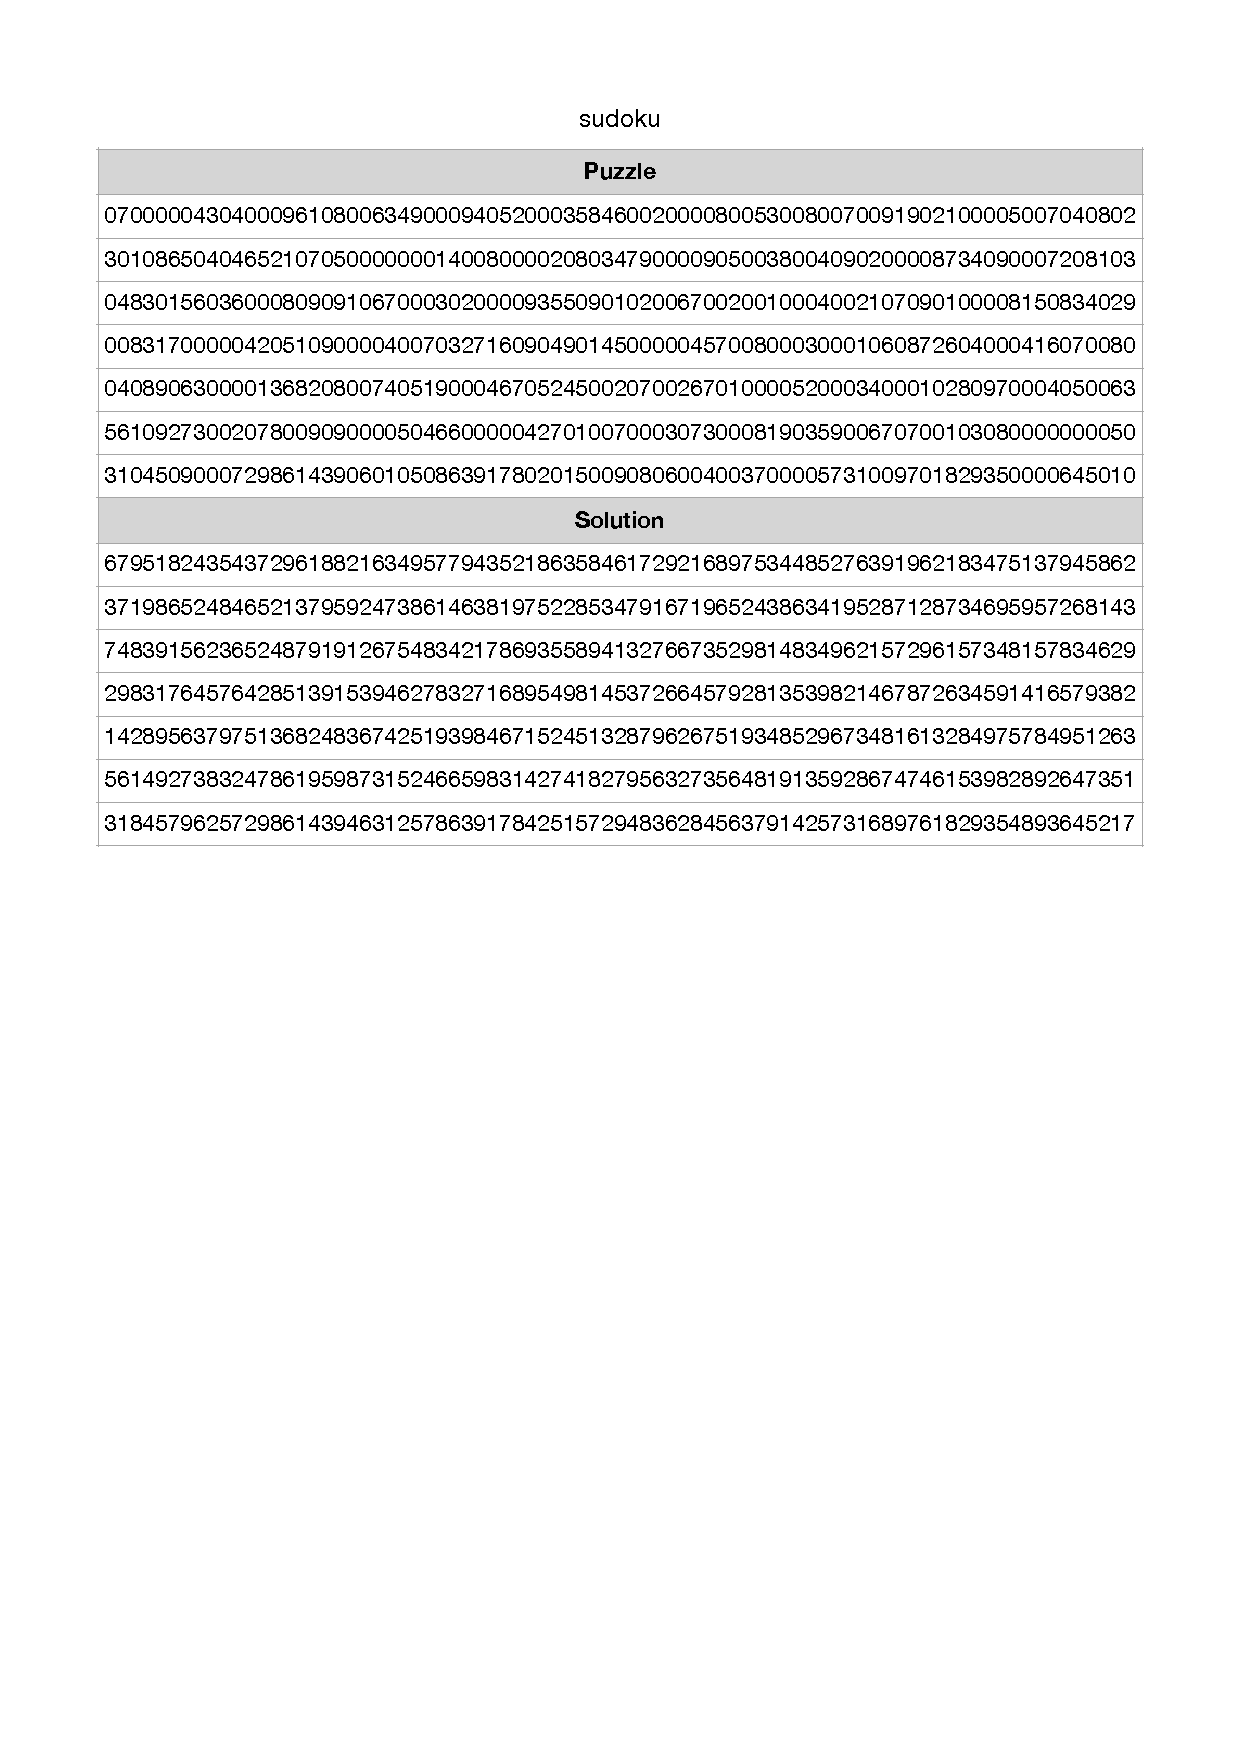
\includegraphics[page=1, width=\textwidth]{figs/sudoku-table.pdf}
    \caption{A sample 9 $\times$ 9 Sudoku puzzle with corresponding solution from the Kaggle 9 Million Sudoku Puzzles and Solutions dataset~\citep{RR:19}}
\end{figure}
\par There are various recent interests in the differentiable neural network for solving the constrained optimization problem~\citep{YF:17, RT:17, WP:19, AB:17}. However, these approaches are targeting a specific problem with the special network structure. Most of them are also not end-to-end learnable models since they focus on the use of continuous parameters for integrating relationships. Is there a general and single end-to-end framework for solving the differentiable optimization in neural network nodes? We argue that the deep declarative network~\citep{SG:19} -- solving the constrained optimization problem -- is a proper and efficient way to approach that. Just as we solve the constrained problem by hand, we believe that it can play the same role in determining the optimal solution. This is the theme of the first part of this thesis. 
\par Let us take a closer look at the more complex problem.  Figure~\ref{fig:chess} shows the possible moves of a Knight in chess, which is not unique and more difficult to determine the optimal solution. Also, the moves are constrained by the positions of other pieces. Therefore, the optimal solution is not guaranteed at this stage. We also have no idea what constraints determine the solution at each step. Is the feasible move restricted to a single point? Or do we have enough information to find the optimal solution? These are the questions we cared about, the regularity of the solution, which is also the theme of the second part of this thesis. 
\begin{figure}[t]
    \label{fig:chess}
    \centering
    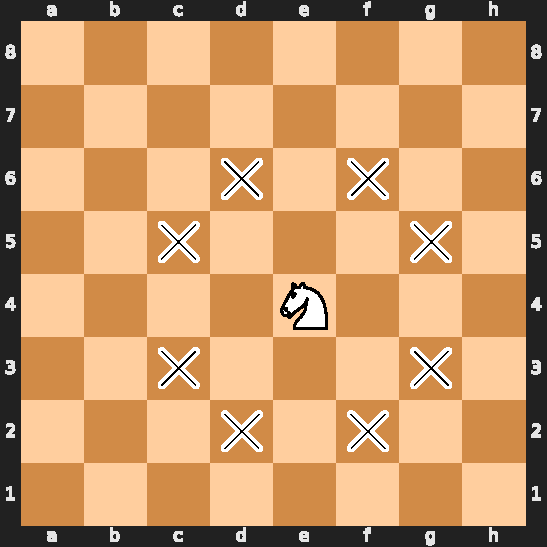
\includegraphics[page=1, width=0.5\textwidth]{figs/chess.pdf}
    \caption{Moves of a Knight, produced from \textit{chess} module in Python}
\end{figure}
\par Therefore, in this thesis, we explore two research directions which employ the deep declarative network as a key component:
\begin{itemize}
    \item \textbf{Multiple constrained declarative nodes} define a general form for different constrained optimization problems and aim to find the gradient solution for them as the output of the layer. 
    \item \textbf{Non-regular solutions in deep declarative nodes} combine and analyze the solution to deal with non-regular points in the solution of the problem. For example, how to approximate the heuristic solution, or solve the constrained optimization problem under different optimality conditions. 
\end{itemize}

\section{Thesis Outline}
\label{sec:outline}
Following the two central themes we mentioned above, this thesis consists of two parts -- PART I Deep Declarative Network: Multiple Constrained Declarative Nodes and PART II Deep Declarative Nodes: Non-regular Solution. 
\par PART I focus on the regular points of multiple constrained declarative nodes in the deep declarative network, with some basic examples of different constraints nodes. 
\begin{description}
    \item In Chapter ~\ref{cha:overviewpart1}, we first give an overview of the theory of optimization, with the discussion of the optimality. Next, we formally define the unconstrained, equality constrained and inequality constrained problems. We then discuss the related works on the solutions to these problems. Finally, the differentiable neural network, an application of numerical optimization in machine learning, is briefly discussed with various modern deep learning algorithms.  
    \item In Chapter ~\ref{cha:ddn}, which is based on works of \cite{SG:19}, we present the details of the deep declarative network. We begin with the overview structure and how it works through the specific declarative nodes. We then introduce the learning progress of the deep declarative network. We analyze the backpropagation through the declarative nodes in different constrained problems. Finally, we give multiple examples of the implementation of the deep declarative nodes in both equality constrained and inequality constrained optimization problems. Also, we point out the limitation of current deep declarative nodes and address some foreseeable ideas for future improvements in the optimization process. We also look to the practical application of the deep declarative network in computer vision tasks.
\end{description}

\par PART II is an extension of the deep declarative nodes in non-regular solution problems, which cannot be solved through the traditional numerical optimization methods. Detailedly, we focus on the approximate solution of the non-regular points with different approaches, which can solve the problem more efficiently. 
\begin{description}
    \item In Chapter~\ref{cha:overviewpart2}, we give an overview of the non-regular solution problems. We list the general non-regular solution cases: overdetermined system, rand deficiency, and non-convex feasible set. We also introduce various related works regarding problems with non-regular gradient results. 
    \item In Chapter~\ref{cha:result}, we demonstrate various possible solutions for each non-regular point case. Since for non-regular solution problems, there are no exact solutions, we can only approximate the closed result. We also compare and discuss the results of each method on minimizing the final loss. Finally, we point out some future works for solving non-regular point problems. 
\end{description}
We will finally present the conclusion in Chapter~\ref{cha:conc}. Proofs for the important theorems and definitions are given in the Appendix.

\section{Contribution}
\label{sec.contribution}
The contributions of this thesis are summarized as follows: 
\begin{itemize}
    \item We implemented the deep declarative nodes with equality and inequality constraints. In particular, we developed nodes for both linear and non-linear constraints based on regular solution points. Examples of each case are also given. 

    \item We made effort to tackle the gradient solution for the non-regular point in declarative nodes. For the overdetermined system, rank deficient problems and non-convex cases, we adequately cover various insightful solutions with simple examples. 
\end{itemize}